\subsection{How to prepare a WSDL document}

Firstly, it should be said that the preparation of WSDL documents 
is nothing that is ultimate fun to do. And it is tricky in the sense that
one does mistakes easily that are difficult to spot.

The community hence started to use computational tools to draft these documents.
The most prominent of these is probably Eclipse.
Since version 3.4 (you might need to install it directly from
\url{http://www.eclipse.org} 
if your distribution is a bit behind or if you are working with Windows)
it offers a web tools platform (WTP) module with which WSDL files can be crafted
graphically.  To install it, point the url http://download.eclipse.org/webtools/updates/
to the Eclipse updater, if it is not already listed.

\subsubsection{Preparation of the Echo WSDL file with Eclipse}

The application starts with a minimal setup, which basically is 
much like the echo web service already. We basically only need to add the
documentation of the service and name the parameters. To do so, just click on
the items displayed in the graphical representation and/or find respective
entries in the tabs below.

\begin{figure}
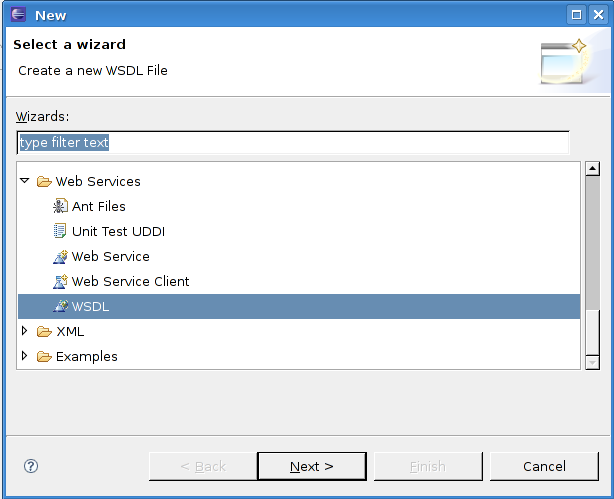
\includegraphics[width=.4\columnwidth]{wsdl_NewFileMenu.png}
\caption{Eclipse dialog to create a new file. WSDL is selected.}
\end{figure}

\begin{figure}
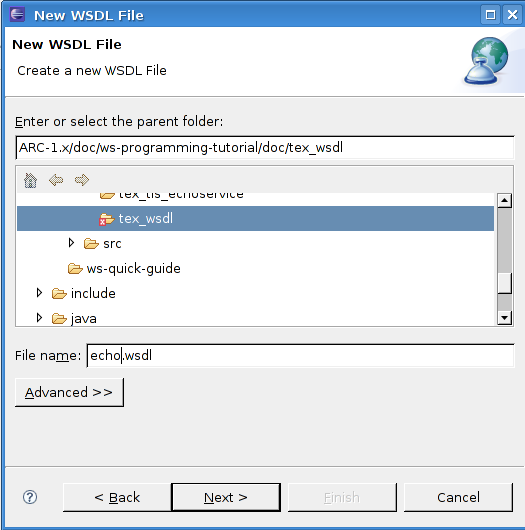
\includegraphics[width=.4\columnwidth]{wsdl_NewWSDLfile.png}
\caption{The default settings are fine for a WSDL service that communicates
with ARC.}
\end{figure}

\begin{figure}
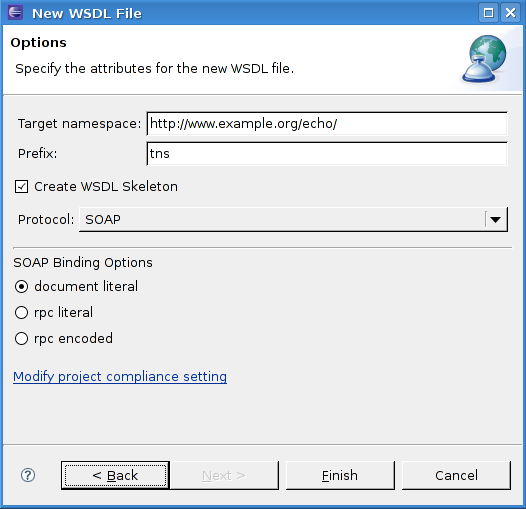
\includegraphics[width=.4\columnwidth]{wsdl_defaultSettings.png}
\caption{The project first shown has already a strong similarity to the Echo
web service that is planned for.}
\end{figure}

\begin{figure}
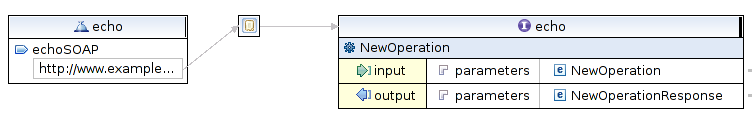
\includegraphics[width=.4\columnwidth]{wsdl_defaultProject.png}
\caption{A first usable web service description is achieved solely by
specifying the address and passing the arguments the known type
\textit{string}.}
\end{figure}

\begin{figure}
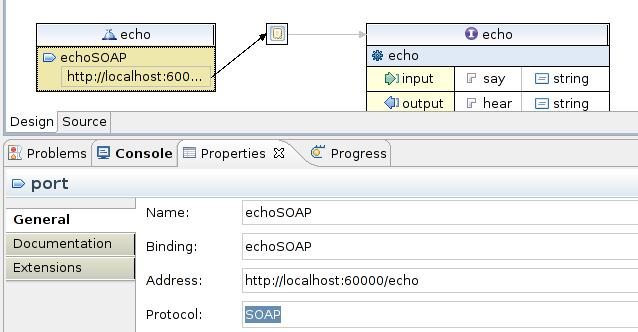
\includegraphics[width=.4\columnwidth]{wsdl_EchoSimplest.png}
\caption{The WSDL for echo in a very simplistic manner.}
\label{fig:simpleEchoService}
\end{figure}

One will fine many specifications that are needed by WSDL to glue the different
parts of the WSDL file together. The service references the bindings and the
bindings reference the port and so on. One should not become overly nervous
about it. The regular programmer does not see those internal names. A good
sanity check for the programmer's view on a WSDL file is to load it from within
the workflow suite Taverna\footnote{Taverna is available from
\url{http://taverna.sf.net}. ARC offers a plugin that allows the direct
communication of Taverna with resources runnign ARC-0. An interface to ARC-1
is still pending. In principle, there is none needed. In practice, we still need
more practice to decide.}.

\begin{figure}
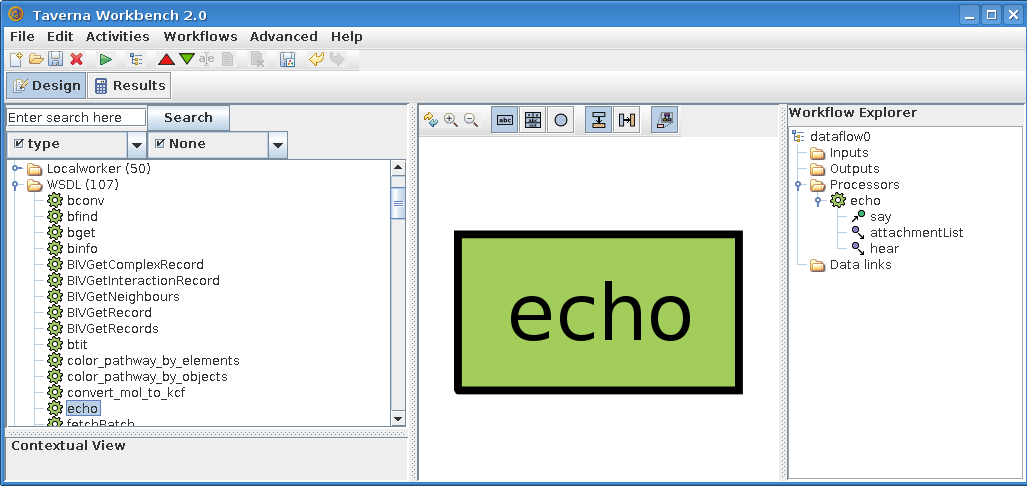
\includegraphics[width=.7\columnwidth]{wsdl_echo_taverna_minimal.png}
\caption{Taverna learned about the Echo Web Service and presents it. No
internal names of WSDL appear, only the name of operations and paramters are
shown.}
\label{fig:wsdlEchoTavernaMinimal}
\end{figure}

The \textit{activities} menu in Taverna offers the item \textit{New Activity}.
It will request the specification of an URL or a local path that points to a
WSDL file. The services presented in there will then be added to the list of
WSDL resources. So will the \textit{echo} workflow that was just prepared with
Eclipse. When it is dragged to the canvas in the middle, as shown in figure
\ref{fig:wsdlEchoTavernaMinimal}, it appears as an interactive object. To the
right, the parameters of the operation are displayed.

\begin{figure}
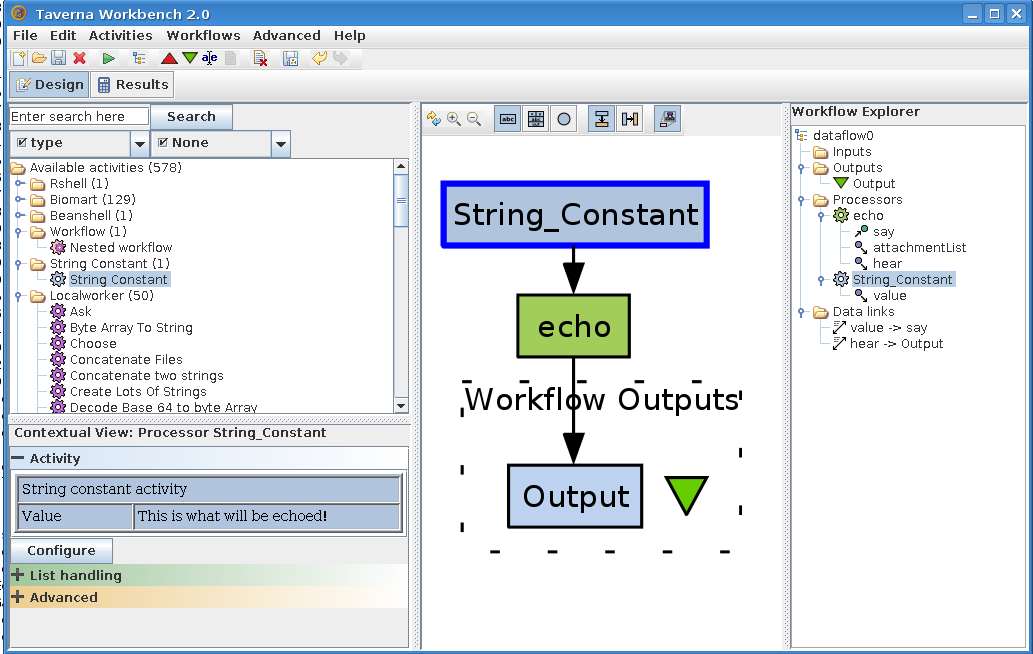
\includegraphics[width=.7\columnwidth]{wsdl_echo_taverna_context.png}
\caption{A completely functional (albeit small) workflow in Taverna that
addresses the Echo Web Service prepared with HED.}
\label{fig:wsdlEchoTavernaContext}
\end{figure}

With a string constant as a constant input added, alternatively one could link a
configurable workflow input as input to the echo Web Service, and the
workflow's output linked as a sink to the output of the workflow, the workflow
is complete. It can now be executed, presuming that the localhost is indeed
running arched with the echo service as described in section
\ref{sec:arch_echo_web_service}.

When comparing the GUI representation of Eclipse as shown with in figure
\ref{fig:simpleEchoService} or that of the just shown Taverna representation
with the raw WSDL of listing \ref{lst:wsdl_eclipse_echo_xml}, it becomes
apparent, that the raw form of the WSDL, as shown below, is more complicated. It seems to invent nested structures that are just not present, since it is only simple strings that are exchanged.
The good news here is, that one would have reached exactly that more
complicated looks when following the original setup without assignment of the
simple type 'string'. WSDL needs special types for every operation. And eclipse
provides them, even when the input types are shown in a more simple manner.


\lstsetECHOECLIPSEXML
\lstinputlisting
	[label=lst:wsdl_eclipse_echo_xml,float=htb,
	caption={[Minimalistic WSDL file for echo created with Eclipse.]
	\textbf{WSDL file for Echo created with Eclipse.}}]
{echo.wsdl}

This has the advantage, that you can use this WSDL file to describe the regular
ARC echo service, even though the original programmer might not have used
Eclipse to create it. Or has he? Gabor?




